\documentclass[10pt,journal]{IEEEtran}

\def\bframe#1\eframe{\begin{frame}#1\end{frame}} %para la tabla
\newcommand\Tstrut{\rule{0pt}{2.6ex}}         % = `top' strut for spacing table
\newcommand\Bstrut{\rule[-1.4ex]{0pt}{0pt}}   % = `bottom' strut for spacing table


\usepackage{siunitx,booktabs,enumitem,array,colortbl,nicematrix}

\usepackage[utf8]{inputenc}
\usepackage[T1]{fontenc}
\usepackage[english]{babel}
\usepackage{amsmath,amsfonts,amssymb}

\usepackage{graphicx}
\usepackage{float} %posicion exacta para las fotos

\usepackage{subcaption}
\usepackage{framed}
\usepackage[noadjust]{cite} %citas agrupadas
%\usepackage{hyperref}
\usepackage{textcomp}  %grados bibliografía

\usepackage{cite}
\usepackage{hyperref}

\usepackage{dcolumn}
\usepackage{tabularx}
\newcolumntype{d}[1]{D{ ,}{.}{#1}} %nuevo tipo de columna con decimales

\usepackage{multicol}
\usepackage{nomencl}
\renewcommand*{\nompreamble}{\begin{multicols}{2}} %para el título del nomencl centrado
\renewcommand*{\nompostamble}{\end{multicols}}
\makenomenclature

\usepackage{subfiles}



\markboth{Journal of Power Sources}{} %titulo pagina
\title{Analysis of structural damage on the struck ship under side collision scenario}


\author{\IEEEauthorblockN{
    Aditya Rio Prabowo \IEEEauthorrefmark{1},
    Dong Myung Bae \IEEEauthorrefmark{2},
    Jung Min Sohn \IEEEauthorrefmark{2},
    Ahmad Fauzan Zakki \IEEEauthorrefmark{3}
    Bo Cao \IEEEauthorrefmark{4},
    and Qing Wang \IEEEauthorrefmark{6}
    },
    \thanks{Received 6 September 2016; revised 11 November 2016; accepted 7 May 2017 Available online 24 September 2017}%
    \thanks{Correspondence:aditya@pukyong.ac.kr}
    \thanks{Peer review under responsibility of Faculty of Engineering, Alexandria University. http://dx.doi.org/10.1016/j.aej.2017.05.002}
    \thanks{1110-0168 ©2017 Faculty of Engineering, Alexandria University. Production and hosting by Elsevier B.V.}
    \thanks{This article is available under the terms of the Creative Commons Attribution License (CC BY).}\\%
\IEEEauthorblockA{\IEEEauthorrefmark{1} Interdisciplinary Program of Marine Convergence Design, Pukyong National University, Busan, South Korea \\}
\IEEEauthorblockA{\IEEEauthorrefmark{2} Department of Naval Architecture and Marine Systems Engineering, Pukyong National University, Busan, South Korea \\}
\IEEEauthorblockA{\IEEEauthorrefmark{3} Department of Naval Architecture, Diponegoro University, Semarang, Indonesia \\}
\IEEEauthorblockA{\IEEEauthorrefmark{4} China Shipbuilding Industry Corporation Economic Research Center, Beijing, China \\}
\IEEEauthorblockA{\IEEEauthorrefmark{6} College of Shipbuilding Engineering, Harbin Engineering University, Harbin, China}
}


\begin{document}
\maketitle

\begin{abstract}
The occurrence of impact needs to be predicted for various cases as it mostly delivers negative to target object and environment. 
In marine structure, this phenomenon has distributed numerous damages to involved objects, such as can be found in tragedy of the Estonia in 1994. This disaster led to a reassessment of the safety of passenger ships in many country. 
During impact both of structural and material aspects contributes to responses in form of energy, force, and damage. 
In present work, consideration of the both aspects would be considered in preparation, analysis, and discussion, to evaluate contribution of considered aspects on failure characteristic. 
A target sub­jected to impact load in form of collision so called struck ship which had different hull configuration would be used in analysis as structural behaviour during and after hull structure of the struck 
ship was penetrated by the striking ship would be observed. In material level, analyses were conducted with applying different mechanical properties on the side structure. 
The results indicated that the tearing of inner hull was avoided due to size of double hull structure. 
This condition provided better safety but lower ship capacity. In other hand, strength characteristic of material was proofed dom-inate difference of internal energy. 
Finally, the influences of material strength, failure strain, and hardening parameter were evaluated and summarized. 
\end{abstract}   

\begin{IEEEkeywords}
Collision scenario; Finite element analysis (FEA); Hull con.guration; Material properties; Internal energy; Crushing force

\end{IEEEkeywords}

%%%%%%%%%%%%%%%%%%%%%%%%%%INTRODUCTION%%%%%%%%%%%%%%%%%%%%%%%%%%%%%%%%%%%%%%%%%%%

\section{Introduction}

\subfile{./01_Introduction/Introduction.tex}

%%%%%%%%%%%%%%%%%%%%%%%%%%%%%%%%%%%%%%%%%%%%%%%%%%%%%%%%%%%%%%%%%%%%%%%%%%%%%%%%%


%%%%%%%%%%%%%%%%%%%%%%%%%%Collision%%%%%%%%%%%%%%%%%%%%%%%%%%%%%%%%%%%%%%%%%%%

\section{Collision phenomenon and material behaviour}

\subfile{./02_Collision/Collision.tex}

%%%%%%%%%%%%%%%%%%%%%%%%%%%%%%%%%%%%%%%%%%%%%%%%%%%%%%%%%%%%%%%%%%%%%%%%%%%%%%%%%


%%%%%%%%%%%%%%%%%%%%%%%%%%Defined%%%%%%%%%%%%%%%%%%%%%%%%%%%%%%%%%%%%%%%%%%%

\section{Defined collision scenario and numerical calculation}

\subfile{./03_Defined/Defined.tex}

%%%%%%%%%%%%%%%%%%%%%%%%%%%%%%%%%%%%%%%%%%%%%%%%%%%%%%%%%%%%%%%%%%%%%%%%%%%%%%%%%

%%%%%%%%%%%%%%%%%%%%%%%%%%Results%%%%%%%%%%%%%%%%%%%%%%%%%%%%%%%%%%%%%%%%%%%

\section{Results and discussion}

\subfile{./04_Results/Results.tex}

%%%%%%%%%%%%%%%%%%%%%%%%%%%%%%%%%%%%%%%%%%%%%%%%%%%%%%%%%%%%%%%%%%%%%%%%%%%%%%%%%

%%%%%%%%%%%%%%%%%%%%%%%%%%Conclusions%%%%%%%%%%%%%%%%%%%%%%%%%%%%%%%%%%%%%%%%%%%

\section{Conclusions}

\subfile{./05_Conclusions/Conclusions.tex}

%%%%%%%%%%%%%%%%%%%%%%%%%%%%%%%%%%%%%%%%%%%%%%%%%%%%%%%%%%%%%%%%%%%%%%%%%%%%%%%%%


%%%%%%%%%%%%%%%%%%%%%%%%%%Acknowledgement%%%%%%%%%%%%%%%%%%%%%%%%%%%%%%%%%%%%%%%%%%%

\section*{Acknowledgement} 

\subfile{./06_Acknowledgement/Acknowledgement.tex}

%%%%%%%%%%%%%%%%%%%%%%%%%%%%%%%%%%%%%%%%%%%%%%%%%%%%%%%%%%%%%%%%%%%%%%%%%%%%%%%%%

\bibliographystyle{IEEEtran}
\bibliography{references.bib}

\begin{figure*}[ht]
    \centering
    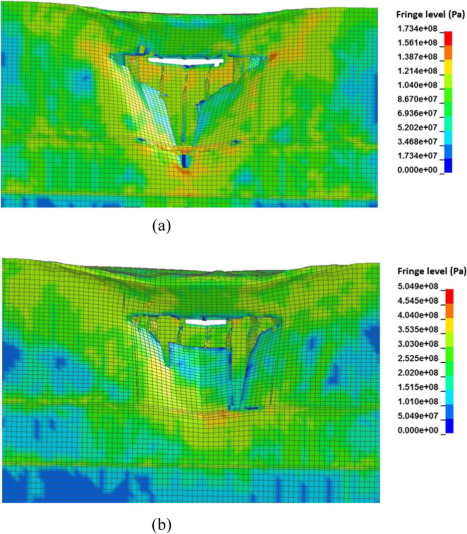
\includegraphics[width=0.5\textwidth]{fig11.jpg}
    \label{fig11}
    \caption{ Damage pattern on the outer and inner hulls: (a) yield 180 MPa, and (b) yield 480 MPa.}
\end{figure*}

    
\begin{figure}[]
    \centering
    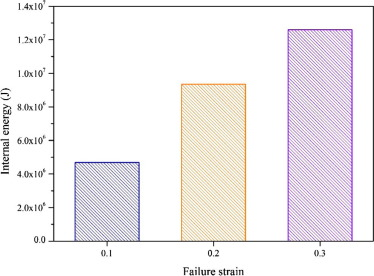
\includegraphics[width=0.9\columnwidth]{fig12.jpg}
    \label{fig12}
    \caption{Effect of failure strain constant to internal energy during ship collision.}
\end{figure}

\begin{figure*}[]
    \centering
    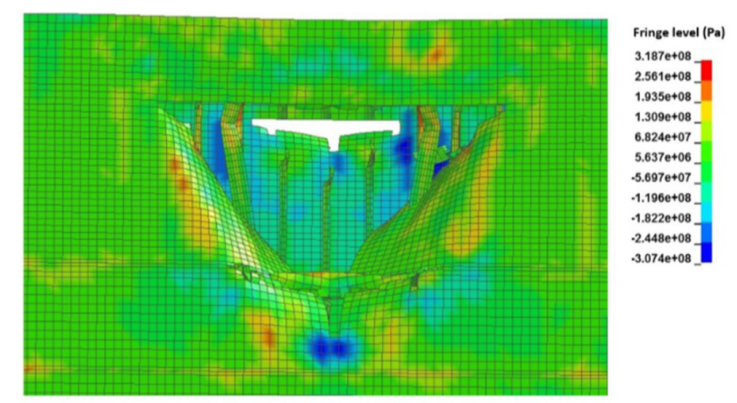
\includegraphics[width=0.8\textwidth]{fig13a.png}
    \label{fig12}
    \caption{Effect of failure strain constant to internal energy during ship collision.}
\end{figure*}

\begin{figure*}[]
    \centering
    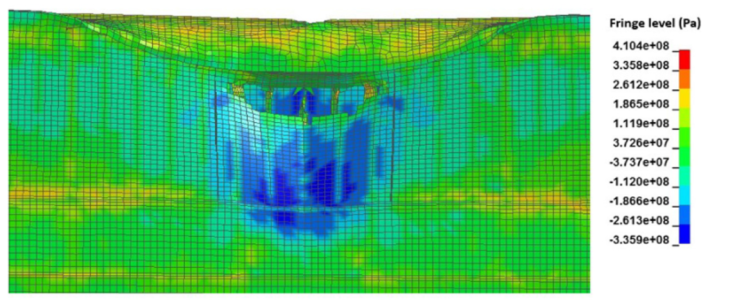
\includegraphics[width=0.8\textwidth]{fig13b.png}
    \label{fig12}
    \caption{Effect of failure strain constant to internal energy during ship collision.}
\end{figure*}

\begin{figure}[]
    \centering
    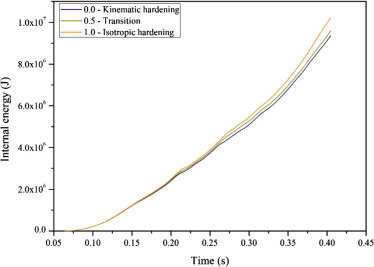
\includegraphics[width=\columnwidth]{fig14.jpg}
    \label{fig14}
    \caption{Internal energy for proposed assumption of yield surface. Significance is not found on the results.}
\end{figure}

\begin{figure}[]
    \centering
    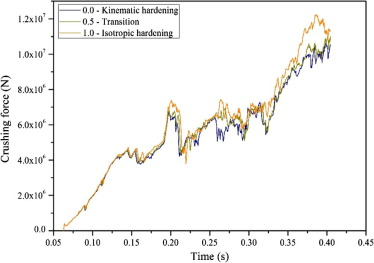
\includegraphics[width=\columnwidth]{fig15.jpg}
    \label{fig15}
    \caption{Crushing force during penetration by the striking ship with different assumed yield surfaces.}
\end{figure}

\end{document}